\documentclass[a4paper, 12pt,twoside]{article}
\usepackage[utf8]{inputenc}
\usepackage[T1]{fontenc}
\usepackage[frenchb]{babel}

\usepackage{lmodern}
\usepackage{textcomp}
\usepackage{ifthen} \usepackage{amsmath} \usepackage{amsfonts} \usepackage{amssymb} \usepackage{graphicx}
\usepackage{enumitem}
\usepackage{multicol}
\usepackage[titlepage,
			a4paper,
			pagenumber,
			sectionmark,
			twoside]{polytechnique}
\usepackage[colorlinks=true,
			linkcolor=black,
			filecolor=red,
			urlcolor=bleu303,
			bookmarks=true,
			bookmarksopen=true]{hyperref}


\title{Projet Scientifique Collectif}
\author{Pierrick \textsc{Allègre} \\
		Gustavo \textsc{Castro} \\
		Clément \textsc{Durand} \\
		Felipe \textsc{Garcia} \\
		Alexandre \textsc{Harry} \\
		Francisco \textsc{Ribeiro Eckhardt Serpa} \\
		Pierre-Alexandre \textsc{Thomas} \\
		Guillaume \textsc{Vizier} \\}
\subtitle{Proposition détaillée}
\date{\today}


\begin{document}
\maketitle
\renewcommand{\baselinestretch}{1.1}
\setlength{\parskip}{0.5em}
\tableofcontents\clearpage

\newboolean{fac}\setboolean{fac}{true}
\newcommand{\vrac}[1]{\ifthenelse{\boolean{fac}}{{\color{red}\itshape #1}}{}}

\section{Introduction du sujet}

	\stepcounter{subsection}
	\vrac{\subsection{Enjeux et motivations}
		Un homme entre dans un hall d’aéroport. Il pose ses valises et s’assoit en attendant l’embarquement. Son  vol  est  en  direction  de  New-York  part  dans  40 minutes. Imitant les gens autour de lui, il sort son smartphone. Il envoie un dernier message à sa femme avant de décoller puis en profite pour prévenir sa maîtresse de son heure d’arrivée. Il consulte alors les derniers résultats sportifs de son équipe de  football  préférée  puis  lit  un  e-mail  de  son  patron. Bien  sûr,  pour  éviter  de consommer son forfait internet, il s’est  connecté  au  réseau  \newcommand{\wifi}{Wi-Fi} \wifi{}  gratuit  proposé dans tous les aéroports, dans tous les lieux publics.
		
		Il ne sait pas qu’en faisant cela, il vient de vous autoriser l’accès à toutes ses données   personnelles:   répertoire,   historique   de   messagerie,   historique   de navigation, voire même ses coordonnées bancaires. Imaginez que vous arriviez à récupérer ces informations. Imaginez tout ce que vous pourriez en retirer. Comme le  confirme  les  dernières  études  à ce  sujet  depuis  maintenant  quasiment  5  ans, notre  smartphone  contient  en  moyenne  plus  d’informations  sur  votre  vie personnelle et professionnelle que n’importe quel autre appareil. Vous venez donc de récupérer assez d’éléments pour faire à peu près ce que vous voulez. Il suffit que cette personne ait un poste plutôt important dans une entreprise pour réaliser que vous détenez des informations précieuses pour un public visé. Vous pouvez même envisagez de faire chanter cette personne. 
		
		Imaginez  maintenant  la situation  opposée.  Vous  voilà  avec  votre  téléphone portable à la Gare du Nord pour un rendez-vous important à Londres. Et voilà que vous vous connectez au \wifi{}. Toutes vos données viennent d’être récupérées par un individu qui pourra s’en servir comme bon lui semble. 
		
		Par  ces  quelques  situations, retranscrites  maintes  fois  dans  les  films d’espionnage, on peut avoir un premier aperçu de ce qu’apporterait la capacité à récupérer les données se trouvant sur un smartphone, jusque parce que celui-ci est connecté en \wifi{}. A partir de cette constatation, nous avons décidé de tester les limites de sécurité d’un smartphone, pour pouvoir par la suite trouver des moyens de le renforcer face à des attaques extérieures.}
		
	\subsection{État de l'art}
	
	Il est possible d'obtenir des données, telles que des mots de passe, via des logiciels comme \newcommand{\wireshark}{\href{https://www.wireshark.org}{WireShark}} \wireshark{} qui écoutent le réseau \wifi{} sur lequel l'appareil cible et celui qui écoute sont connectés. Avec \wireshark{} on peut écouter tous les paquets IP de l'autre utilisateur connecté au \wifi{} et on sauvegarde \vrac{toute} l'information qu'il transmet dans le but d'obtenir des informations de tout type. On peut exploiter certains protocoles qui transmettent des données  peu ou pas cryptées et ainsi décoder les messages qu'ils véhiculent. Des attaques possibles sont: 
	
	\begin{itemize}\setlength{\parskip}{0pt}
		\item DNS\footnote{Domain Name System, service permettant de traduire un nom de domaine en informations de plusieurs types qui y sont associées (adresses IP, etc.)} Poisoning : le hackeur se fait passer pour un serveur DNS. Lorsque l'utilisateur envoie une requête au serveur, il reçoit une réponse éventuellement manipulée et ne le sait pas. 
		\item ARP\footnote{Address Resolution Protocol, traduisant une adresse réseau en une adresse physique} Poisoning
		\item "Man in the middle" attack : cette attaque est fréquemment utilisée par les pirates. Un attaquant pénètre dans le dispositif (la conversation) et intercepte les données pour les exploiter ou les modifier avant de les laisser passer vers leur destination finale.
		\item Eavesdropping : capture et décodage du trafic d'une application pour obtenir des informations
		\item AP Phishing\footnote{Hameçonnage} : consiste en l'imitation d'un serveur web, par exemple pour se faire passer pour la page d'un site bancaire et récupérer des mots de passe, etc.
	\end{itemize}

	Il \vrac{est$\rightarrow$était} également possible de faire des attaques via SMS ou MMS pour hacker le portable. L'attaque consiste en l'envoi d'un message avec une vidéo qui exploite la vulnérabilité de la librairie \verb!stagefright! sur \newcommand{\Android}{Android} \Android{}, qui est une librairie utilisée pour traiter les fichiers multimédia.\vrac{(ajout) Cette faille a été découverte et comblée récemment.}

	Des procédés existent déjà pour sécuriser les échanges et les données qui sont mises en danger par les éléments précédents.
	
	La plupart des smartphones utilisent des applications pour sécuriser les données dans le téléphone, comme par exemple les antivirus. Le problème est parfois que l'antivirus ne travaille pas à un niveau logiciel suffisamment bas pour totalement sécuriser le mobile. Il existe aussi l'option consistant à crypter les données stockées dans le téléphone.
	
	Pour sécuriser les données transmises via \wifi{}, SMS ou \newcommand{\bluetooth}{Bluetooth} \bluetooth{}, il y a des applications servant à crypter les messages, comme par exemple \href{http://www.whispersystems.org/#encrypted_texts}{TextSecure}. On utilise aussi le SSL\footnote{Secure Sockets Layer} pour crypter le trafic de certaines applications. Ces solutions sont locales et souvent payantes ou contraignantes.

	\vrac{
	\subsection{Objectifs}
		Notre objectif final est double. Nous voulons dans un premier temps mettre en  évidence  la  possibilité  d’obtenir  des  informations  censées  être  sécurisées. Depuis un ordinateur portable, notre but est «d’espionner» un appareil \Android{} connecté au même \wifi{}. Nous pourrons observer les différentes failles de sécurité grâce à cette première étape. Cette  démarche débutera par une analyse de ce qui peut être récupérer «passivement» par l’ordinateur, puis nous tenterons d’accéder à encore plus de données en organisant une attaque sur l’appareil test.
		
		Dans un deuxième temps, nous utiliserons l’expérience accumulée dans la phase «hacking» afin de créer, sûrement sous forme d’application, une façon de mieux  protéger  les  données  personnelles  contenues  sur  les  smartphones.  Notre objectif ici n’est pas de rendre le smartphone invulnérable à toute attaque, mais au  moins  d’encapsuler  les  informations  de  telle  sorte  à  ce  que  l’accès  à  celles-ci soient relativement plus compliqué pour un intrus.}

\section{Organisation du projet}

	\subsection{Méthode d'organisation}
	
	Le groupe a mis en place différents systèmes et règles destinées à garantir une bonne organisation et à nous permettre de remplir au mieux nos objectifs. Une organisation structurée, claire et précise est en effet importante pour permettre à notre projet d'avancer le mieux possible.
		
		\subsubsection{Division du travail}
		
		Régulièrement le groupe sera divisé en petits groupes pour mieux répartir le travail. Cela signifie en particulier qu'il n'est pas toujours nécessaire que le groupe se réunisse au complet pour discuter de certains sujets attribués à un petit groupe.
		
		Nous avons considéré important, chaque fois que l'on fonctionne en petit groupe, de désigner un responsable qui facilitera la communication et la coordination au sein du groupe complet.
		
		\subsubsection{Rendez-vous}
		
		Si les groupes travaillant sur une tâche commune communiqueront et se rencontreront régulièrement et souvent pour avancer, il est tout de même important qu'aient lieu suffisamment souvent des rendez-vous. C'est pourquoi le groupe a convenu de se réunir au complet, avec le tuteur de stage et l'encadrant, une fois toutes les trois voire deux semaines.
		
		Ceci n'exclut pas des éventuels rendez-vous supplémentaires lorsque cela est nécessaire, mais de tels rendez-vous réguliers sont importants pour s'assurer que tout le monde a une vue globale sur le projet et pour faire le point de façon efficace sur notre progression.
		
		\subsubsection{Communication}
		
		Des règles claires de communication sont importantes pour tous fournir un travail bien coordonné. Une liste de diffusion sera mise en place pour que chaque mail soit transmis à tous les membres du groupe, cela incluant évidemment le tuteur de stage et le cadre référent.
		
		Nous avons convenu d'utiliser la plateforme de bloc-notes collaborative \href{https://framapad.org}{framapad} en guise de tableau d'affichage nous permettant de partager les informations et notes importantes tout au long de l'année. Il permet d'afficher les contributions de chacun tout en les distinguant, le tout en temps réel. Le même développeur\footnote{Framasoft, association loi 1901} propose d'ailleurs un service d'organisation de rendez-vous, \href{https://framadate.org}{framadate}, que nous utilisons aussi pour simplifier le choix des dates de réunion afin d'être tous présents aux rendez-vous.
		
		Nous ne pourrons tout de même pas nous réunir chaque fois que nous en aurons besoin, compte tenu des emplois du temps de chacun. Cette impossibilité éventuelle d'être physiquement réunis pour discuter du projet a été anticipée, et nous avons mis en place un canal — ou salon — de discussion IRC\footnote{Internet Relay Chat} permettant de mettre en place d'éventuelles réunions virtuelles de façon simple.
				
		\subsubsection{Distribution des rôles}
		
		\paragraph{"Chef" de groupe. } Pour faciliter le fonctionnement du groupe, \textcolor{bleu303}{Guillaume \textsc{Vizier}} sera chargé tout au long de l'année de jouer un rôle de coordinateur dans le groupe. C'est l'expéditeur privilégié des mails d'informations, et il se charge en général d'organiser les rendez-vous ou de distribuer certaines tâches. Contrairement à ce que laisse penser l'appellation, il ne s'agit pas d'une position d'autorité dans la mesure où les membres du groupe travaillent en collaboration : ce rôle consiste en particulier à clarifier et transmettre des décisions prises en commun, et à faciliter la coordination du groupe.
		
		\paragraph{Édition des documents. } Pour assurer la cohérence et l'uniformité des documents produits par le groupe, \textcolor{bleu303}{Clément \textsc{Durand}} sera chargé de mettre en commun les contributions à chaque document. Cela permet principalement de produire des compte-rendus de réunion communs, de rassembler les informations constituant chaque document, et de se charger de la mise en page des documents après avoir collecté toutes les parties.
		
		\paragraph{Logistique. } Pour que le groupe fonctionne dans de meilleures conditions, \textcolor{bleu303}{Gustavo \textsc{Castro}}, \textcolor{bleu303}{Felipe \textsc{Garcia}}, et \textcolor{bleu303}{Franscico \textsc{Ribeiro Eckhardt Serpa}} se chargeront de l'organisation pratique des différents rendez-vous. Réserver des salles, s'assurer des disponibilités de chacun, feront notamment partie de leurs prérogatives.
	
	\subsection{Échéancier}
	
	À partir des échéances imposées par la Direction des Études, de notre objectif principal et des informations que nous avons sur l'objet d'étude, nous avons mis en place une chronologie prévisionnelle destinée à préciser nos objectifs et notre organisation. Cette liste d'objectifs intermédiaires et de tâches permettra de donner une ligne de conduite. Elle peut toutefois être révisée au fur et à mesure, pour être adaptée à notre progression et à d'éventuels changements d'objectifs dûs à nos découvertes ou difficultés. Elle a l'avantage de clarifier la vision qu'a chacun du projet, et de tous nous mettre d'accord sur ce que nous souhaitons précisément faire.
	
		\subsubsection{Objectifs intermédiaires du groupe}
		
		\paragraph{Première partie. } Pour atteindre nos objectifs, c'est-à-dire produire un dispositif logiciel permettant de sécuriser certains aspects du fonctionnement des smartphones, il faut commencer par comprendre ce fonctionnement et ces failles.
		
		Nous souhaitons commencer par comprendre les failles « naturellement » présentes, c'est-à-dire les informations divulguées (fuites) par un téléphone ou tout autre dispositif, sans qu'une personne tierce n'agisse pour faciliter ces fuites. L'objectif est d'être capable de capturer ce qu'il se passe sur un réseau, pour pouvoir observer ce que les appareils diffusent dans leurs échanges. Il serait alors intéressant de constater l'importance des fuites, pour mettre en évidence le manque de sécurité au travers de toutes les informations non cryptées qui circulent dans un réseau, qui sont transmises par des applications.
		
		La suite logique des choses nous conduirait à étudier de façon statistique ces données présentes en quantité très importante, étudier la force du cryptage de celles qui sont cryptées, pour être capable de mettre en évidence quel type d'information est directement accessible et diffusé par nos appareils de communication. Enfin, serait évidemment instructif d'étudier les protocoles d'échange utilisés dans les réseaux pour en apprendre plus sur ce que peut faire un hacker, ce à quoi il peut avoir accès. Le DNS poisoning est un des exemples d'attaque dangereuse pour les utilisateurs, et pourtant simple pour les hackers.
		
		L'objectif de cette partie est de mettre en évidence et de faire constater la présence de risques importants en terme de vie privée, que ce soit sur les réseaux sociaux ou même sur des applications n'ayant a priori aucun lien avec nos informations personnelles. Cela justifie notre choix d'objectif en mettant en évidence l'utilité de ce que nous souhaitons produire, et sera un moyen pratique de s'instruire sur le domaine que nous étudions, d'apprendre les nouveaux langages dont nous avons besoin et le fonctionnement des protocoles que nous rencontrerons.
		
		\paragraph{Seconde partie. } À partir de cette étude des failles des appareils de communication de la vie courante, l'objectif principal du groupe est de combler ces failles dans certains cas, qui seront précisés ci-après.
		
		Nous avons décidé de nous concentrer — au moins dans un premier temps — sur les appareils Android. Essentiellement des téléphones portables, ils diffusent des informations très variées en quantité impressionnante, et présentent d'importantes failles. L'objectif de cette partie est donc de réduire ou combler certaines de ces failles.
		
		Dans un premier temps, nous souhaitons réaliser une application dont le fonctionnement principal importe peu, mais dont les données sont sécurisées. Le but est d'avoir une application qui respecte la vie privée de l'utilisateur, et protège les données qui lui sont confiées. Cela nous permettra d'étudier la possibilité de combler le manque de \emph{cloisonnement} entre les applications installées sur un téléphone, lequel manque est source de nombreuses fuites au sein même du téléphone. L'utilisateur ne veut en effet pas que les données qu'il confie à une applications soient récupérées par une autre sans son accord explicite, et le but de cette étape est de répondre à ce problème. Une fois les données sécurisées au sein du téléphone, le but est de sécuriser les échanges de données.
		
		À ce moment nous aurons alors produit une application simple mais a priori plus sécurisée que ce que nous aurons constaté auparavant sur la plupart des applications. Le but est ensuite de généraliser cette sécurisation aux autres applications. Il s'agira alors de créer une application ou un programme qui protègera les données de l'utilisateur contre les failles que nous avons découvertes. Cette application pourra par exemple crypter les échanges d'informations entre utilisateurs soucieux de leur sécurité, protéger le téléphone contre d'éventuelles irrégularités de comportement du réseau, limiter et mieux contrôler les informations qui sont diffusées de façon non cryptée, etc. Cette étape, qui est essentiellement notre objectif principal, est conséquente et nous procéderons par étapes comme suit.
		
		\begin{itemize}\setlength{\parskip}{0pt}
			\item Décider des failles que nous souhaitons combler et de la façon de les combler.
			\item À partir de cela, étudier ce qu'il faut être capable de contrôler sur le téléphone et en déduire le format (langage, position par rapport aux autres applications, etc.) de notre application.
			\item Éventuellement revoir nos objectifs en fonction de ce qu'autorise ou non la programmation sur le téléphone.
			\item Coder une application réalisant ces objectifs.
		\end{itemize}
		
		Enfin, une fois cette application terminée, nous pourrons étudier les failles du système équipé de notre programme. C'est l'un des intérêts de notre première partie, car nous pourrons utiliser les outils utilisés ou conçus durant notre étude de la sécurité des appareils de communication pour étudier l'utilité de l'application produite. Il sera en effet intéressant d'avoir étudié les données diffusées par un téléphone neuf, par un téléphone contenant des applications dites « de confiance » ou au contraire des applications réputées pour ne pas respecter la vie privée, pour les comparer (en terme de quantité d'information disponible) à celles diffusées par un téléphone équipé de ce que nous aurons produit.
		
		\subsubsection{Confrontation aux échéances}
		
		Ces objectifs sont à intégrer dans le calendrier de déroulement du PSC prévu par la Direction des Études.
		
		\paragraph{Réunion de lancement. } Cette réunion doit avoir lieu au plus tard le 20 novembre 2015. L'objectif est d'avoir à ce stade une bonne connaissance du sujet en ayant commencé la première étape et étudié les différents domaines que nous allons rencontrer. Une meilleure connaissance de ce que nous étudions nous permettra d'avoir une bonne vision du sujet, de ce que nous pouvons faire, et d'être le plus réalistes et efficaces possible.
		
		\paragraph{Rapport intermédiaire. } À la date de remise du rapport intermédiaire, le 15 janvier 2016, nous souhaitons avoir terminé et exploité la première étape, ainsi que commencé la seconde. Cela nous permettra d'avoir des résultats intermédiaires concrets, et une réelle connaissance du sujet.
		
		La précision de ces échéances et de notre calendrier nous permettra au fur et à mesure de préciser nos objectifs, de les compléter ou éventuellement de les réviser, en évitant d'être dépassés par le temps ou la difficulté.
			
	\section{Moyens à disposition et résultats préliminaires}
	
		\subsection{Moyens nécessaires}

		Notre sujet concernant la sécurité du système d'exploitation Android à travers ses communications (particulièrement en \wifi{}), nous allons avoir besoin de plusieurs éléments pour compléter nos objectifs.
		
		La liste n'est pas exhaustive, et au fur et à mesure de notre avancement il est fortement probable que de nouveaux logiciels ou même du matériel supplémentaire soient nécessaires.
		
		Bien évidemment nous aurons besoin de téléphones ou tablettes supportant Android, nous prévoyons dans un premier temps d'employer nos propres appareils, mais nous n'excluons pas de demander des emprunts ponctuels au laboratoire si le besoin s'en fait sentir.
		
		Ensuite pour la partie « Mise en évidence de vulnérabilités », nous allons avoir besoin de nombreux logiciels (notamment des sniffeurs de paquets). Comme nous essayons en partie de montrer que ces vulnérabilités sont accessibles à tout individu averti mais sans expertise particulière, la plupart de ces logiciels sont gratuits et même parfois \emph{opensource}\footnote{Code source ouvert}. Pour effectuer les tests, nos ordinateurs personnels seront amplement suffisants pour le début de nos objectifs.
		
		Enfin, tout au long de notre progression nous allons avoir besoin de documentation. Évidemment, étant donné le caractère sensible de ce que nous comptons effectuer, il est relativement difficile de trouver des ressources, et encore plus difficile de trouver des ressources à jour. En effet le domaine de la sécurité informatique est en développement constant et de nombreuses failles sont corrigées chaque jour.

		Pour l'instant nous utiliserons ce que nous arrivons à trouver en ligne et avec l'aide de notre tuteur. Si cela se révèle ne pas être suffisant, nous aviserons en temps voulu avec son aide.

		\subsection{Résultats préliminaires}

		Comme nous l'avons mentionné plus haut, nous allons utiliser des sniffeurs de paquets ou autres outils d'analyse réseau pour récupérer et traiter les échanges de données effectués par l'appareil.
		
		De tels logiciels existent déjà, notons par exemple iftop, Netstat et enfin \wireshark{} (voir figure \ref{pic:wireshark}) que nous avons déjà commencé à prendre en main et avec lequel nous prévoyons d'effectuer la première partie de notre travail.
		
		\begin{figure}[!ht]
		\centering
		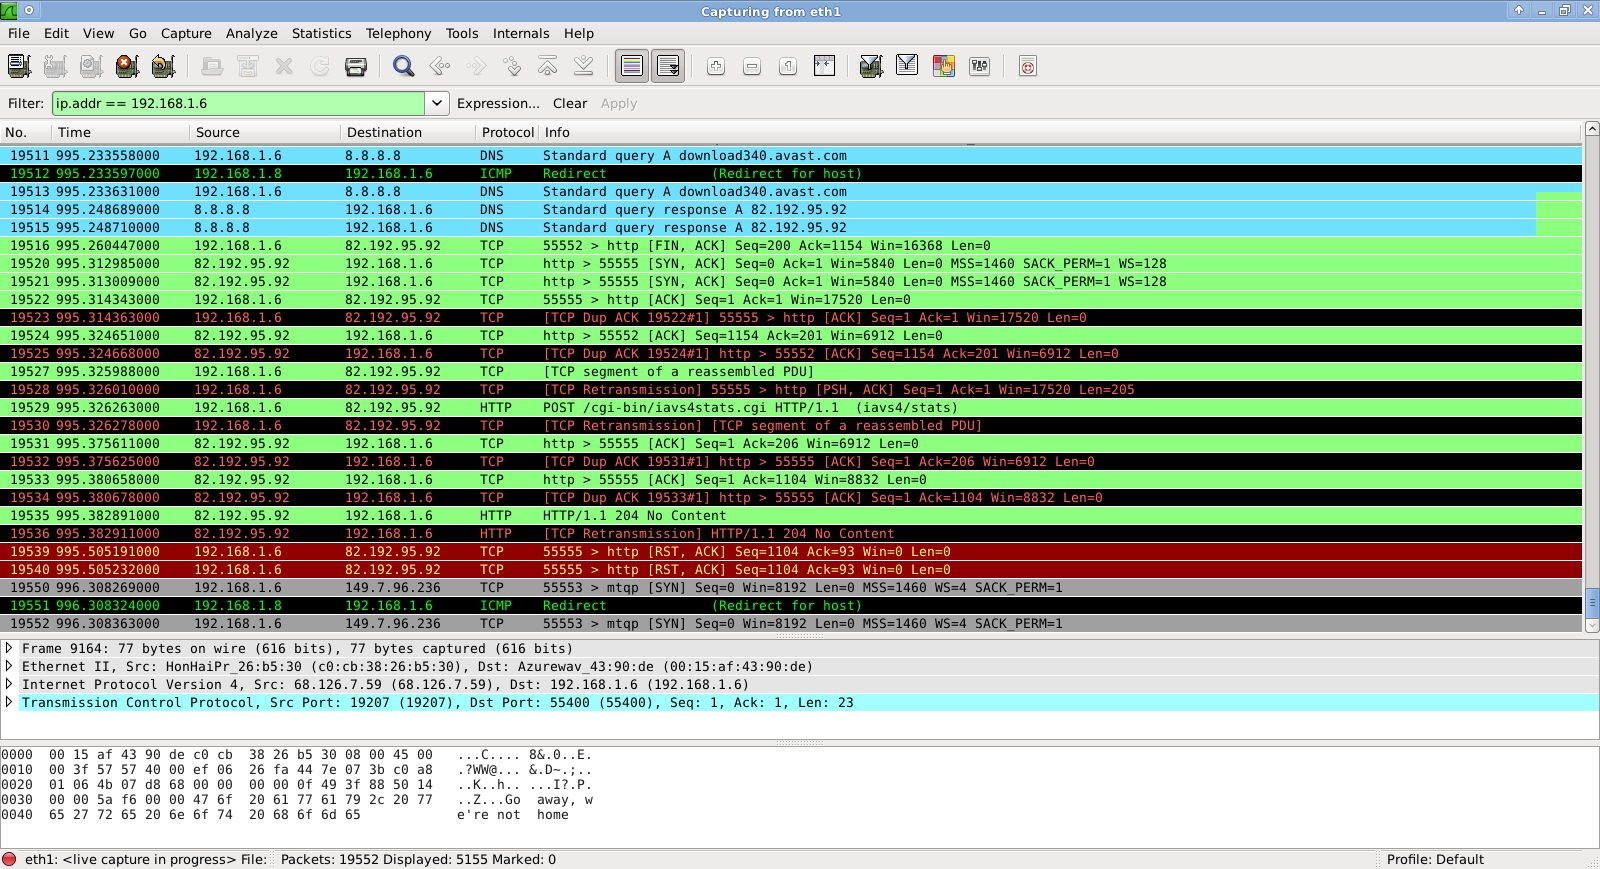
\includegraphics[width=0.8\textwidth]{wireshark.jpg}
		\caption{L'interface du logiciel WireShark}
		\label{pic:wireshark}
		\end{figure}
		
		Notre tuteur de stage nous a déjà confirmé qu'il était possible d'analyser les données échangées pour récupérer des informations (que ce soit dans le but de faire du social engineering et/ou pour effectuer une attaque active après coup), parfois même ces informations peuvent être la cible.
		
		\clearpage % la bibliographie seule sur une page ?
		\subsection{Références bibliographiques}
		{
		\renewcommand{\section}[2]{} % pour virer le titre "Références"
		\nocite{*}
		\bibliographystyle{plain}
		\bibliography{proposition_detaillee}
		}

\end{document}